\documentclass[11pt]{article}
\usepackage[a4paper,margin=1in,marginparsep=0pt,marginparwidth=0pt]{geometry} %showframe
\usepackage[xetex]{graphicx} % Required for inserting images
\usepackage{eso-pic}
\usepackage{url}
\usepackage[dutch,english]{babel}
\usepackage[colorlinks=true]{hyperref}
\usepackage{xcolor}
\usepackage{tikz}
\definecolor{nlesc-blue}{RGB}{0, 157, 221}
\definecolor{nlesc-purple}{RGB}{53, 6, 57}
\definecolor{nlesc-yellow}{RGB}{255, 178, 19}

\usepackage{caption, booktabs}
\usepackage{multirow}
\usepackage{ltablex}

\usepackage{tabularray}
\UseTblrLibrary{booktabs}
\newcommand{\testtable}[0]{
\begin{booktabs}{colspec={rccc},row{odd}={blue9}}
    \toprule
    Thing & Value & Value & Value\\
    \midrule
    A & 1 & 2 & 3\\
    B & 1 & 2 & 3\\
    C & 1 & 2 & 3\\
    \specialrule{2.5pt,teal5}{1pt}{1pt}
    D & 1 & 2 & 3\\
    E & 1 & 2 & 3\\
    \bottomrule
\end{booktabs}
}

%\newcommand{\mythinline}{\noalign{\hrule height 0.8pt}}

\newcommand{\placelogo}[0]{
\AddToShipoutPictureBG{%
%  \AtPageLowerRight{\makebox[1.3\textwidth][r]{%
%    
\includegraphics[scale=1]{img/a0000-img003.jpg}}}}
\AtPageUpperLeft{\raisebox{-8\baselineskip}{\makebox[\paperwidth]{\hspace{16cm}
\includegraphics[scale=1]{img/a0000-img002.png}}}}
  \AtPageLowerLeft{\raisebox{2\baselineskip}{\makebox[\paperwidth]{\hspace{16cm}
\includegraphics[scale=1]{img/a0000-img003.jpg}}}} 
}%
}

\usepackage{fontspec}
\defaultfontfeatures{Mapping=tex-text,Scale=MatchLowercase}
\setmainfont{Nunito}

\usepackage{titlesec}
\titleformat{\section}{\color{nlesc-blue}\fontsize{18}{20}\bfseries}{\color{nlesc-blue}\thesection}{1.5em}{}
\titleformat{\subsection}{\fontsize{16}{18}\bfseries}{\thesubsection}{1.5em}{}

%\titleformat{\section}{\fontsize{11}{15}\bfseries}{\Roman{section}}{1.5em}{USI }

\title{{\fontsize{36}{38}\selectfont \textbf{\color{nlesc-purple}Project Management Protocol of the Netherlands eScience Center}}}
\author{Authors: Netherlands eScience Center Programme Managers}
\date{Date: September 2023\\Version: 2.0}

\begin{document}

\hypersetup{,urlcolor=blue,citecolor=blue,linkcolor=blue}

\begin{titlepage}

\AddToShipoutPictureBG*{%
  \AtPageLowerLeft{\makebox[1.32\textwidth][r]{%
    
\includegraphics[scale=1]{img/a0000-img001.png}}}}


        \maketitle


  
            
\begin{table}[!h]
\resizebox{1.1\textwidth}{!}{%
\begin{tabular}{llc}
\multicolumn{1}{c}{Date} & \multicolumn{1}{c}{version} & Changes   \\
1 October 2023           & 2.0 updates                 & \multicolumn{1}{l}{\begin{tabular}[t]{@{}l@{}}DT and PM mandates, Roles of Directors, PMs role in Ambition 2,\\ SS, KD and external projects, Communications role, Editorial team, \\ breakdown of hours, opportunities beyond project, \\ Technology Status Report, End report\end{tabular}} \\
23 September 2022        & 1.0 initial version         &                                                                                                                                                                                                                                                                                           
\end{tabular}%
}
\end{table}
            
  %      \vspace{0.8cm}




\end{titlepage}

\clearpage
\setcounter{tocdepth}{2}
\tableofcontents

\clearpage

\placelogo{}
    
\section{Scope and definitions}
\label{sec:scope}

\subsection{Scope}

This document is the official project management protocol for the Netherlands eScience Center. It describes all phases
of a project and the procedures required to successfully complete them.

The scope of this document is the execution of research projects awarded by the eScience Center through calls for
proposals, though other types of projects are also briefly covered. This document gives a detailed description of all
steps, both necessary and optional, that must or may be taken in the execution of projects, reflecting the so-called
\textit{project life cycle}. For each step, the document indicates the responsibilities of the project team members
(RSEs) and other eScience Center employees (e.g. Programme Managers, Finances, Directors Team) involved in the
process.

Call procedures follow a separate protocol~\cite{call-protocol-2015} and are
not covered by this document. The call procedure protocol ends with the formal awarding of projects by the eScience
Center Governing Board or the Directors Team (DT), the notification of Lead Applicants and the formalization of the
awarding by means of a \textit{toekenningsbrief} ('Awarding letter’). The
current document describes all activities that (need to) take place from that moment onwards, until the formal closing
of the project. An independent evaluation of projects, including impact, output, process and collaboration with project
partners is outside of the scope of the current document, and will be published as a separate document or a subsequent
version of this document in the future. 

This document has been approved by the DT and will be subject to evaluation and possible adaptation annually.

The structure of this document largely follows the project life cycle (see Section~\ref{sec:scope:lifecycle}); the
protocol describes activities in chronological order.

\subsection{Stakeholders}
An eScience project is a project involving the eScience Center, where responsibility is shared between different
stakeholders who each have their own roles and responsibilities during specific phases of the project.


%\resizebox{\textwidth}{!}{%
%\begin{tabular}{p{0.15\textwidth}p{0.15\textwidth}p{0.2\textwidth}p{0.2\textwidth}p{0.1\textwidth}}
\begin{tabularx}{\linewidth}{p{0.12\textwidth}|p{0.12\textwidth}|p{0.12\textwidth}|p{0.25\textwidth}|p{0.25\textwidth}}%{@{}lX@{}}
%\caption{My caption} \\
\toprule
\textbf{Stakeholder} & \textbf{Abbreviation} & \textbf{Assignment}& \textbf{Role}& \textbf{More info}\\
\midrule
\endfirsthead
\toprule
\textbf{Stakeholder} & \textbf{Abbreviation} & \textbf{Assignment}& \textbf{Role}& \textbf{More info}\\
\midrule
\endhead
\midrule
\multicolumn{5}{r}{}
\endfoot
\bottomrule
\endlastfoot  
Lead Applicant                                     & LA                    & main applicant and recipient of the grant                                                                         & primary contact for the eScience Center project, accountable for the (quality of the) scientific contribution to the project                                                                                                           & responsibilities defined in the call text, the Terms and Conditions document, and potentially a Consortium/Collaboration agreement.  \\\hline
Programme Manager                                  & PM                    & assigned by the PM team~\footnote{All PMs, led by the Programme Director, constitute the PM team.}                                                                                          & accountable for the eScience contribution to a project, responsible for realization of project results given predetermined resources and timelines, project budget holder                                                              & Full text of responsibilities available in the PM job profile document (see Section 5 for the reference) and PM mandate (Appendix~\ref{app:sec:pm-mandate}) \\\hline
Lead Research Software Engineer                    & Lead RSE              & appointed by accountable PM                                                                                       & responsible for the timely execution of the project, main contact person for the project with other stakeholders                                                                                                                       & More details on responsibilities, see the formal role description of Lead RSE (Appendix~\ref{app:sec:leadRSE}).                                          \\\hline
Research Software Engineer (assigned to a project) & RSE                   & assigned by the accountable PM                                                                                    & responsible for the timely completion of the project                                                                                                                                                                                   & All RSE activities coordinated by Lead RSE in agreement with PM.                                                                     \\\hline
Consulting Research Software Engineer              & Consulting RSE        & involved at request of Lead RSE or accountable PM                                                                 & responsible for contributing expertise to a project for a limited but predetermined time, can be involved in some of the key meetings, in addition to an expertise contribution                                                        & All activities coordinated by Lead RSE in agreement with PM in case the project team needs additional expertise.                     \\\hline
Technology Lead                                    & TL                    & assigned by the TL team~\footnote{All TLs, led by Director of Technology, constitute the TL team.}                                                                                          & acts as point of contact for Lead RSE to the TL team. Safeguards the technological aspects of a project; accountable for the quality, reuse and sustainability of the research software developed.                                     & The TLs team is responsible for internal training programme of RSEs.                                                                 \\\hline
Section Head                                       & SH                    & assigned by the PM/SH team~\footnote{All SHs, led by Executive Director, constitute the SH team.}                                                                                       & line manager of RSEs, responsible for monitoring the overall effectiveness of RSEs in bringing projects to completion; maintain overview of a research domain.                                                                         & The SH team assigns one SH to each RSE team, and the SH ensures that team keeps its capacity and planning up to date.                \\\hline
Communications                                     &                       &                                                                                                                   & advise and facilitate internal and external communications of projects, including but not limited to showcasing projects through news items, website, newsletters, social media, interviews and videos.                                &                                                                                                                                      \\\hline
Community Manager                                  & CM                    &                                                                                                                   & advise on developing outreach activities and promoting community engagement, responsible for external training programme                                                                                                               &                                                                                                                                      \\\hline
Secretary                                          &                       &                                                                                                                   & organizes formal meetings, provide with agenda and slide template, invitation text, list of participants (with emails), and timeline.                                                                                                  &  \href{mailto:secretaries@esciencecenter.nl}{secretaries@esciencecenter.nl}                                                                                         \\\hline
Programme Director                                 & PD                    &                                                                                                                   & the escalation point for PMs, the contact point of PMs to DT for project related changes that need the DT decision, approves the workshops plans (in the agreement with F\&C on the financial part). The budget holder of Acquisition. &                                                                                                                                      \\\hline
Director of Technology                             & DoT                   &                                                                                                                   & The escalation point for TLs, the contact point of TLs to DT, accountable (and responsible) for licences and Intellectual Property (IP), software sustainability budgets holder                                                        &                                                                                                                                      \\\hline
Director of Operations                             & DoO                   &                                                                                                                   & handles legal questions (e.g., contracts, Collaborative Agreements and guest agreements)                                                                                               &                                                                                                                                      \\\hline
Finance \& Control                                 & F\&C                  & part of Operations, includes Controller, and led by DoO                                                           & responsible for maintaining financial project administration in Exact                                                                                                                                                                  & \href{mailto:finance@esciencecenter.nl}{finance@esciencecenter.nl}                                                                                            \\\hline
Directors Team                                     & DT                    & comprised of DoT, DoO, General Director and PD                                                                    & approves formal decisions regarding projects (e.g., budget changes)                                                                                                                                                                    &                                                                                                                                      \\\hline
GDPR contact person                                &                       & appointed by the DT, see the intranet for contact information                                                     & consults on GDPR~\cite{GDPR} or privacy-related issues in the project                                                                                                                                                                             & The eScience Center has not appointed a Data Protection Officer. GDPR aspects must be discussed with the contact person.             \\\hline
eScience Center project team                       & eScience project team & comprises RSEs, PM and TL working on the project                                                                  & responsible for the timely completion of the project                                                                                                                                                                                   &                                                                                                                                      \\\hline
Project team                                       &                       & comprises the eScience project team, LA and their team (including team members indicated in the project proposal) & responsible for the timely completion of the project                                                                                                                                                                                   &                                                                                                                                      \\\hline
Editorial Team                                     &                       &                                                                                                                   & provides support with outreach                                                                                                                                                                                                         & The eScience Center maintains a blog, and has presence in major social networks                                                     
%\end{tabular}%
%}
\end{tabularx}


\subsection{Types of projects}
The eScience Center receives an annual budget from NWO and SURF, the larger part of which is allocated to projects
submitted by researchers working at eligible research performing organizations in the Netherlands in the form of the
in-kind provision of RSEs. Projects may also be funded from external sources (henceforth referred to as \textit{an
external project) }or funded from the annual budget but carried out internally.

By awarding subsidy to a project or by pledging a contribution to an external project, the eScience Center takes on the
obligation to deliver high-quality work in a timely manner.

\subsubsection{Call projects}

The eScience Center publishes a range of calls. Each project is a part of a specific call (regular calls such as
OEC/ASDI, CIT/DTEC/eTEC/JEDS, SSI, or calls in collaboration with other funders such as ADAH, Big Data \& Health, GO,
JCER, eTEC-BIG, ESI-FAR). Projects from the regular calls before 2021 are partly in-cash, while projects awarded later
are fully in-kind (plus a reserved budget for workshops).

Calls can reserve part of the project or the call budget to serve the eScience Center agenda to increase the impact of
software beyond the project itself. Henceforth this will be referred to as the software sustainability budget, formerly
known as generalization budget). The budget is intended for software generalization, reuse and sustainability, and
community building. The DoT is the holder of this budget. Details concerning this budget are included in the Awarding
letter. See Section~\ref{sec:opportunities:softsust} for more information.

Project teams (mainly Lead RSE, PM and TL) are expected to consult the specific call text, Awarding letter
(‘Toekenningsbrief’), Terms and Conditions document (‘Bijzondere voorwaarden’, ‘Subsidieregeling’, etc.), Consortium/Collaboration Agreement (CA), and/or
contracts for grant terms and conditions. The LA is responsible for adhering to the conditions of the project, while
the PM, with the help of the Lead RSE, monitors this.

In our call projects, most of the total requested budget is dedicated to project work and project-related activities.
The remaining part (referred to as “general activities”) covers activities that benefit our ability to contribute to
high-quality research, such as the professional development of RSEs through training, work meetings, conferences, etc,
as well as the administrative coordination and project management within the eScience Center. It is up to the PMs and
RSEs in consultation with the SHs to fairly distribute hours for general activities across all the projects they
contribute to (cf. Section~\ref{sec:exec:budget}). The exact percentage set aside for general activities is defined in
the call within which a project has been awarded.

\subsubsection{External projects}

Projects funded externally by e.g. NWO or the EU, or via private-public partnerships, are governed by external funding
conditions specified in a contract or agreement that may supersede our own rules. The budgets of these projects need to
be approved by F\&C and the DoO. Again, the project team (mostly, Lead RSE, PM, TL) must consult the specific call
text, Awarding letter, Terms and Conditions document, Consortium/Collaboration Agreements, contracts for the conditions
and rules. The LA is responsible for adherence to the rules and conditions, while the PM with the help of the Lead RSE
monitors this. Projects under external funding are covered partially by this protocol.\footnote{A budget for writing
grant proposals for external funding, use of it follows the process described in “External funding” (see Section
\ref{sec:opportunities:external-funding} for more information).}

\subsubsection{Other projects}

This document only briefly covers other types of projects such as those funded through Ambition 2, namely Dissemination
\& Community (D\&C), Knowledge \& Development (KD)\footnote{cf. Netherlands eScience Center strategy~\cite{nlesc-strategy} to get familiar with the term.} and Fellowship projects in 
Section~\ref{sec:opportunities:fellowship} and Appendix~\ref{app:pm-role}.

\clearpage
\subsection{Project life cycle overview}
\label{sec:scope:lifecycle}

\begin{figure}[!h]
    \centering
    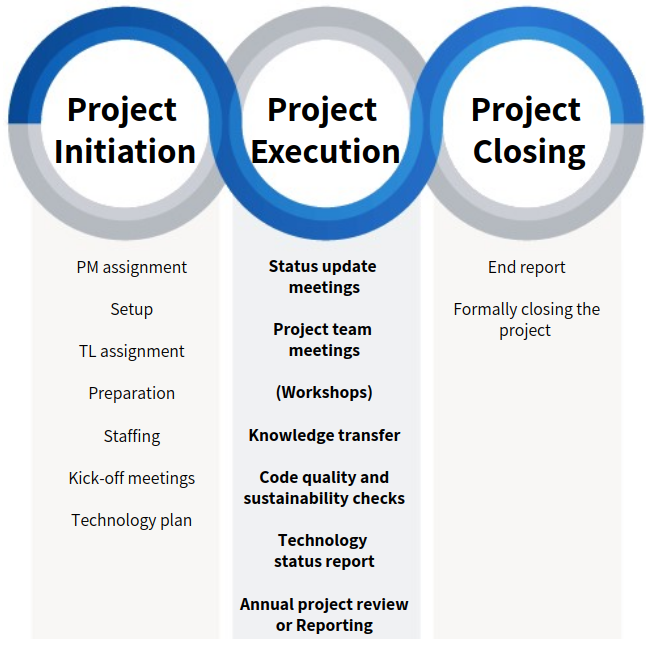
\includegraphics[scale=0.5]{img/lifecycle-stages.png}
    \caption{Project lifecycle stages}
    \label{fig:project-lifecycle}
\end{figure}

At the eScience Center, a standard project life cycle is a three-phase process (see Figure~\ref{fig:project-lifecycle}). First, project stakeholders initiate the
project. Next, the project team executes the project and monitors its progress. Finally, once the project reaches its
end, it is formally closed.

These three phases are covered in detail in the next sections.

\clearpage
\section{Project Initiation}
\label{sec:init}
The project initiation phase starts immediately after the project has been granted. Its goal is to set up the project
within the eScience Center, including a planning in terms of staffing and a work plan.

For \textbf{external projects} and projects from specific calls (e.g., collaborative calls), F\&C ensures that all
paperwork is in place (e.g., contracts, Consortium/Collaborative Agreements, Memorandum of Understanding) before making
a project active in Exact, allowing RSEs to write hours spent on the project. The PD regularly keeps PMs up to date on
outstanding applications for external funding, signals to PMs and F\&C whenever a project has been granted, and hands
over relevant documents (such as proposal, agreements made, preliminary budget, etc) to PMs. 

PMs are accountable for call projects. For the \textbf{external projects}, PMs assign a PM and Lead RSE to the project
(i.e., the RSE involved in the submission procedure). Together with the Lead RSE the PM works with the project partners
to get all paperwork in order (such as a subcontract), cf. Section~\ref{sec:init:legal}. 

\subsection{PM assignment}
Each project has one accountable PM. The PM team assigns PMs to new projects at the first PM meeting following the
granting decision, records the assignation and asks F\&C to update Exact with new budget holder information (the newly
assigned PM). If agreement over an assignment is not reached, the PD makes the final decision in their capacity as PM
team chair.

Should the accountable PM become unavailable for an extended period, the PM team can decide to put another PM in charge
of the project.

\textbf{Responsible: PM team.}

\subsection{Administrative Setup}
The table offers an overview of the responsibilities of the different stakeholders in setting up a project:

\begin{table}[!h]
\begin{booktabs}{colspec={|>{\bfseries}p{0.15\textwidth}|p{0.15\textwidth}|p{0.65\textwidth}|},row{even}={nlesc-yellow}}
\toprule
\textbf{What} & \textbf{By} & \textbf{Responsible for}  \\[2ex]
Exact  & F\&C  &
    \begin{minipage}[t]{0.65\textwidth}
    \begin{itemize}\itemsep0em
        \item Creating project code
        \item Entering and uploading attachments
        \item Making PM budget holder 
    \end{itemize} 
    \end{minipage}  \\[2ex]
Project portfolio on SharePoint~\cite{proj-portfolio}  & F\&C  & 
    \begin{minipage}[t]{0.65\textwidth}
    \begin{itemize}\itemsep0em
        \item Creating folder in project portfolio (with template subfolder \& documents)
        \item Uploading granting package documents (incl. Awarding letter), signed start form, CA if applicable
    \end{itemize} 
    \end{minipage}  \\[2ex]
\multirow{2}{*}{Research Software Directory (RSD), project page and software pages} & PM             & \begin{tabular}[c]{@{}l@{}}Creating an RSD project page9, putting placeholder image with the eScience logo10 \\ Signalling requirements for corporate website to Communications \\ Copying website summary from the proposal (if applicable) or writing a summary and obtaining approval from LA for edited versions  \\ Finding appropriate image (e.g., royalty-free images offered by shutterstock.com and unsplash.com) \\ Ensuring Lead RSE has a maintainer access to the RSD page\end{tabular} \\
                                                                                    & Communications & Advising and reviewing content for the pages, including editing summaries, supporting with images                                                                                                                                                                                                                                                                                                                                                                                                     \\
Corporate website  & Communications &  
\begin{minipage}[t]{0.65\textwidth}
    \begin{itemize}\itemsep0em
        \item Ensuring content is displayed on the corporate web page with information supplied by PM
        \item Promoting projects to target stakeholders, when relevant. Promotion may include but is not limited to news items, inclusion in newsletters and social media
    \end{itemize} 
    \end{minipage}  \\
Ganttic  & PM             & 
\begin{minipage}[t]{0.65\textwidth}
    \begin{itemize}\itemsep0em
        \item Checking if import project information from Exact is correct 
        \item Adding labels
        \item Adding respective project portfolio URLs
        \item Planning RSEs, if applicable (e.g., for external projects)
    \end{itemize} 
    \end{minipage}  \\                    
    \bottomrule
\end{booktabs}
\end{table}


\textbf{General status and progress are monitored by the accountable PM.}

\subsection{TL assignment}
The PM asks the TL team to assign a TL to the project, providing all project information. The TL team does so at the TL
meeting and informs the PM of their decision (by assigning TL to the project in Ganttic as well as a confirmation by
email). Should the assigned TL become unavailable for an extended period, the TL team assigns another (temporary) TL to
the project.

\textbf{Responsible: TL team (at request of the PM).}

\subsection{Preparation by PM}
PM provides an overview of project requirements based on the project proposal, covering the following topics:

\begin{itemize}
\item What technology/eScience expertise is requested from the eScience Center, and at what level (novice, expert)?
\textbf{Action}: In collaboration with the TL, the PM prepares relevant tags for technologies required by the project.
\item What are the research questions and goals? \textbf{Action:} PM asks senior members of the Center with relevant domain
expertise for their opinion and prepares relevant tags for the project information.
\item What is the proposed workplan and timeline? Is the work feasible? \textbf{Action}: Together with the TL, the PM assesses
if a workplan is feasible or needs to be adjusted in the context of the Technology plan (Section~\ref{sec:init:techplan}).
\item What type of support other than RSE expertise is requested and needed? (e.g., training workshops, time and help of CMs,
use of SURF or other infrastructure) \textbf{Action}: PM notes this information for discussion with the LA and Lead
RSE. PM consults TL about management plans (see Section~\ref{sec:exec:mp}) and CMs about training workshops (see
Section~\ref{sec:exec:training}).
\end{itemize}
PM flags issues such as:
\begin{itemize}
\item GDPR – is there any personally identifiable information involved in the data required by the project? 
\item IP and licensing – does the project team ask for an exception to the Apache 2.0 and the CC by 4.0 default? 
\item Long term sustainability of the software – does the project have a sustainability plan? 
\item Anything else potentially problematic – for example, military application, animal or human tests, etc. (see also the
final statements in the application form).
\end{itemize}

Depending on the issue, PM contacts relevant consultants (see Section~\ref{sec:exec:consult}).

PM records all relevant information in the project log (Section~\ref{sec:exec:log}).

\textbf{Responsible: accountable PM}



\subsection{Staffing}
PM assigns the project to a team and appoints a Lead RSE in agreement with SHs and budget
holders relevant to the team activities. The PM can adjust staffing at any point during the project life cycle
whenever necessary.

PMs normally assign a project in such a way that it does not involve more than one team, unless no team is willing to
take up the project. The Lead RSE is the primary contact for the project.

PMs assign RSEs to projects, taking the RSEs' expression of interest (see Section~\ref{sec:init:vacancy} below) into account, and following due consultation with relevant stakeholders such as SHs,
TLs, RSEs and teams. 

PM communicates staffing decisions to the LA. 

\subsubsection{Project vacancy announcement}
\label{sec:init:vacancy}
Project vacancies are announced internally at the discretion of the \textbf{accountable PM} in a timely manner,via email. An announcement message must contain an instruction on how to access information on the project and how to
express interest (filling out form, via email, comments on Announcement Board in Teams etc.). In turn, RSEs express
their interest (also on behalf of their team) within the allocated time and provide a motivational text including
expertise and skills relevant to the project work. PM informs RSEs on staffing results.

If there is a shortage of RSE expertise and the project cannot be staffed, the PM signals the vacancy to the respective
SH and the PM representative in the hiring committee following rules described in the hiring process~\cite{hiring-intranet}.


\subsubsection{Assignment of RSEs}
To find RSEs suitable for the project, the PM:

\begin{itemize}
\item reviews the RSE expressions of interest,
\item checks availability of RSEs,
\item consults other PMs and the relevant SHs and TLs.
\end{itemize}

The PM assigns RSEs based on RSEs' expressions of interest, availability, technological skills and
disciplinary match. If a team of RSEs is assigned to a project, the PM and the team agree as to which member(s) and in
which capacity they work on the project. Team members are free to distribute the workload, but the Lead RSE role cannot
be freely transferred. Although each project has only one Lead RSE, team members are collectively responsible for all
the projects assigned to them, and are expected to help each other towards the successful completion of their
projects.

The Lead RSE plays a leading role in the project execution phase. The PM assigns the Lead RSE in consultation with the
relevant SH, based on (amongst others) seniority and/or potential. The PM consults the relevant SH regarding the
professional and/or personal development needs of the Lead RSE.

The Lead RSE and PM use email for all official correspondence with the project team (including the LA), keeping each
other in CC. This includes information regarding any significant change concerning the project (budget, deliverables,
changes in research team), agreements on management plans (DMP, SMP), workshops, review meetings and end reports.

\subsubsection{Lead RSE availability}
If the Lead RSE has limited availability during the project for an extended period, this is signalled to the PM and the
SH by the Lead RSE. The PM discusses with the SH whether the Lead RSE should be temporarily or permanently replaced.
The eScience project team puts forward a candidate to take up the role of Lead RSE.

The PM approves replacement of a Lead RSE. In normal circumstances, the former Lead RSE organizes a transfer meeting
with the new Lead RSE and the PM, and reports on the status of the project (current workplan, tasks, responsibilities
of all project RSEs and the next steps in the project execution), ensures proper RSD pages handover. The PM
communicates the change to the LA (or Consortium for external projects) and includes both the former Lead RSE and the
new Lead RSE in the correspondence.

\subsubsection{Project Planning}

Project planning in Ganttic is used as an agreement between the PMs and the RSEs. RSEs are expected to adhere to the
planning as agreed; if required, they can discuss and renegotiate the planning with the PMs.

To plan projects, PMs rely on information available in Ganttic. SHs ensure that information on the availability of RSEs
for at least the next 6 months is up to date; this includes the overall planning overview of an
RSE's activities, such as trainings, extended leave, etc. Other work done by RSEs (Dissemination
\& Community; Knowledge Development) are filled in by the respective budget holders. The PM (in consultation with F\&C)
ensures the planning leads to the project staying within its budget.

To make planning of projects more robust, PMs schedule RSEs on a yearly or quarterly rather than a monthly/weekly/daily
timescale, on the assumption that project hours are spent at a constant rate throughout all projects. In collaboration
with SHs and relevant budget holders, the PMs ensure that no RSE is planned beyond their capacity; should this be the
case, assignments are removed in agreement with the RSE and SH so that capacity is on par.

To facilitate a robust planning across projects and RSEs, PMs discuss the planning of each team at least once every
quarter, in a meeting including the SH associated with the team. The Lead RSE can propose planning of the project.

PMs share the resulting planning with the organization (e.g., through Ganttic).


\subsection{Kick-off meetings}
Once administration and staffing are finalized, the PM organizes two kick-off meetings: an administrative start meeting
introducing the eScience Center and our way of working and a project kick-off, which is focused on the project research
and workplan. The secretary can assist with organizing the meetings.

The PM archives the material used during the meeting and the meeting notes (from LA, PM or others) internally in the
project portfolio folder.

The PM can combine the two meetings, if necessary, into a single workshop-style meeting. This applies in particular to
specific categories of projects (e.g., based on a collaborative call, or an OpenSSI call). This is held at the eScience
Center office, and a suitable room is arranged by the PM.

For \textbf{external projects}, the way kick-off meetings are arranged depends on the nature of the project. The Lead
RSE attends all formal meetings of external projects. The PM joins these meetings if they deem this necessary. It is
the responsibility of the Lead RSE to keep the PM in the loop.

\subsubsection{Administrative start meeting}

\begin{table}[!h]
\begin{booktabs}{colspec={|>{\bfseries}p{0.15\textwidth}|p{0.85\textwidth}|},row{even}={nlesc-yellow}}
    \toprule
    Scheduled: &  Soon after awarding, but not before the Awarding letters have been sent and F\&C has collected all the paperwork and put it in Exact and Project Portfolio). \\[1.5ex]
    Stakeholders: & PM (chair), LA, Lead RSE (optional). The PM can involve others at their discretion. \\[1.5ex]
    Purpose: &  A procedural meeting to discuss how the cooperation on this project will be organized, administrative questions the LA may have, current availability of software and data, staffing, etc, so that problems can be caught early (e.g., licensing issues, no data, etc.). \\[1.5ex]
    Duration: & 1.5 hours \\[1.5ex]
    Location: & At the eScience Center (preferably), but can be also online. \\[1.5ex]
    \bottomrule
\end{booktabs}
\end{table}

For this meeting, the PM uses the administrative (PowerPoint) presentation, ensuring that information is in the line
with the call text, and current Terms, IP policies etc.

The agenda for this meeting covers:

\begin{itemize}
\item The eScience Center
\begin{itemize}
\item its mission, governance structure, technological expertise
\item request to sign up for the eScience Center newsletter
\item request to follow the eScience Center social media channels for latest updates.
\end{itemize}
\item Working with the eScience Center
\begin{itemize}
\item calls, collaboration, software and software quality, RSD
\item what are the roles of PM, Lead RSE, RSEs, teams and TL
\item suitable and welcoming work environment~\cite{arbo} for RSEs at the project location, including
working-on-location permit ('gastovereenkomst')
\item additional collaboration options: workshops, trainings, other calls.
\end{itemize}
\item Project life cycle
\begin{itemize}
\item workshops organized by the project
\item annual reviews, reports, payments
\item Project end
\item SURF Support for the projects (infrastructure, advisors).
\end{itemize}
\item Community and impact
\begin{itemize}
\item RSD, project pages, pitches, etc
\item publishing, blog posts, and outreach activities
\item digital skills programme
\item contributions to open and reproducible science initiatives.
\end{itemize}
\item Intellectual Property and Software Licenses
\begin{itemize}
\item publication protocol: funding acknowledgement in output is a must, RSEs are preferably co-authors
\item any deviation from the default IP policy (open source from the start, not only after release).
\end{itemize}
\item Project introduction
\begin{itemize}
\item project needs and expertise
\item Software and data readiness (Software and Data accessibility and quality checks).
\end{itemize}
\end{itemize}

The PM logs the agreements reached in the slides or the project log (Section~\ref{sec:exec:log}). The PM updates the
project log with the meeting date, stakeholders present and (link to) the agreements. The PM and LA share slides with
each other and the PM stores both slide decks (from PM and LA) and agreements in the project portfolio.

\subsubsection{Project Kick-off}

\begin{table}[h!]
\begin{booktabs}{colspec={|>{\bfseries}m{0.15\textwidth}|m{0.85\textwidth}|},row{even}={nlesc-yellow}}
    \toprule
    Scheduled: &  Around the date indicated by LA in the start form, after the administrative start meeting. \\[1.5ex]
    Stakeholders: & PM (chair), the entire project team, TL, and other relevant stakeholders (e.g., SH)  \\[1.5ex]
    Purpose: &  The project kick-off focuses on the execution of the project, on the technological requirements, scientific challenges, relevant communities, project goals and outputs. \\[1.5ex]
    Duration: & Max. 1.5 hours \\[1.5ex]
    Location: & At the eScience Center office or at the institute of the LA\footnote{Mandatory participants of a meeting be present in-person at the office, while all optional participants can also participate via video conferencing if they prefer.} \\[1.5ex]
    \bottomrule
\end{booktabs}
\end{table}

For this meeting the standard agenda is:

\begin{itemize}
\item Round of introductions (the entire project team) (10 min)
\item Project introduction and goals by LA (20 min)
\item Discussion on the workplan and any updates needed by the project team (30 min)
\begin{itemize}
\item eScience team explains the purpose of the technology plan
\item Project team in agreement with the PM and TL, decides when the technology plan should be submitted
\end{itemize}
\item Roles of the project team members in carrying out the project workplan (10 min)
\item (Updates to) Software Management Plan (SMP) and Data Management Plan (DMP) (5 min)
\item Agreements on initial project planning and deliverables (with concrete action points) (10 min)
\item Agreements on collaboration (e.g. frequency and location of project team meetings, planning days to work together and
location)
\item Any other business (5 min).
\end{itemize}

A workplan should always include a clear set of steps, divided into work packages, a detailed and realistic schedule, a
list of deliverables and management plans (see details in Section~\ref{sec:exec:mp}).

In agreement with the project team, the Lead RSE prepares the project for the code development (see details in Section~\ref{sec:exec:code}). PM logs the agreements, asks LA for the slides, and archives all of it in the project
portfolio.


\subsection{Technology plan}
\label{sec:init:techplan}

The project team submits a technology plan by the date agreed during the project kick-off, describing
\begin{itemize}
\item possible choices of the available technologies and which of them will be used for the project, and for which reason
\item the technological outcomes of the project (software and data) 
\item steps to be taken regarding reusability and adoptability, etc. 
\end{itemize}
The technology plan covers the choice of programming language(s), expected quality levels, etc. The plan should be seen
as an evolving record of the considerations and choices regarding the technology employed; it ensures that RSEs make
good use of the expertise present in the Center and that optimal choices are made throughout the project. An example of
project technology plan is included in the Appendix~\ref{app:exampleplan}.

\begin{table}[!h]
\begin{booktabs}{colspec={|>{\bfseries}m{0.2\textwidth}|m{0.8\textwidth}|},row{even}={nlesc-yellow}}
    \toprule
    Written by: &  Lead RSE, in collaboration with project team (including LA, TL), CMs, and others RSEs or colleagues (e.g. with relevant expertise on the subject), or relevant SIG. \\[1.5ex]
    Target audience: & Project team, TLs, PMs  \\[1.5ex]
    Schedule: &  %
    \begin{minipage}[t]{0.8\textwidth}
    \begin{itemize}\itemsep0em
        \item written at the start of the project work, before any software development starts,
        \item submitted to PM/TL by email before the deadline agreed during the project kick-off, 
        \item as a part of the project log (either full document in the log or a URL to it). 
    \end{itemize} 
      \end{minipage}
    \\[1.5ex]
    Approved by: & PM after due consultation of TL. \\[1.5ex]
    \bottomrule
\end{booktabs}
\end{table}

The Lead RSE is encouraged to reach out to RSEs or other colleagues who have the relevant expertise in the process of
developing the technology plan. CMs can advise on engaging the target audience with regard to software reusability and
adoptability. Since TLs are accountable for safeguarding the suitable technology in the project, the involvement of the
TL in writing the technology plan is important. Therefore, the PM must consult the TL on the technology plan, submitted
by the Lead RSE before any technological decisions are made in the project.

Upon approval of the technology plan (via email), the project team updates the management plans, if necessary. The Lead
RSE logs the decisions in the project log (see Section~\ref{sec:exec:log}) and archives emails in the project
portfolio, if necessary. The Lead RSE keeps the technology plan up to date: if it changes during the project, this
should be simply appended to the original technology plan (e.g., in a separate document or in the project log). The
Lead RSE explains why adaptations to the plan were required. The aim is to obtain a record of the lessons learned from.
beginning to end of the project, to facilitate collaboration and to document decisions in case a project must be
transferred to other RSEs due to unforeseen circumstances. The Lead RSE discusses any changes made to the technology
plan during the status update meetings (Section~\ref{sec:exec:status}).

\subsection{Legal agreements}
\label{sec:init:legal}
The eScience Center champions and supports open and reproducible science and open-source development. Lead applicants
get their projects awarded under the eScience Center's Terms and Conditions~\cite{nlesc-terms}. The default agreement forms offered by universities often contain IP related provisions that contradict
our Terms and conditions.

Regardless of the type of the project, RSEs must not sign any formal agreement document prior to consulting the PM. Such
documents include but are not limited to:
\begin{itemize}
\item Guest agreement (to get guest status at the project partner organization)
\item Data sharing agreement
\item IP related document
\item Consortium agreement
\item Collaborative agreement
\item Non-disclosure agreement
\end{itemize}

PM checks the draft agreement document and decides whether it can be signed and informs the RSE. If needed, the PM can
consult PD. The RSE archives the final signed version of the agreement in the project portfolio.

PM and PD signal to the DoO if legal advice is required. In that case, any proposed contracts are sent to the DoO by the
PM for final approval. The DoO shares the information within F\&C.

\clearpage
\section{Project execution}
Projects at the eScience Center vary in duration from 3 months to 5 years, depending on the call through which they were
granted. In all call projects, the PM (with the help of Lead RSE) monitors progress of the project and involves
relevant stakeholders whenever necessary. The Lead RSE takes on a leading role during the execution phase of the
project life cycle. The Lead RSE ensures that the Project team meetings take place on a regular basis: the frequency
may vary with the size of the team, e.g. full team meetings once per month and meeting with only with the LA and/or LA
team once in two weeks.

\subsection{Project logging}
\label{sec:exec:log}
eScience project team members routinely log important project events and agreements. The project log is placed in the
Project portfolio (the Coordinators subfolder, see Appendix~\ref{app:folders}). The Lead RSE keeps the log up to
date (see example in Appendix~\ref{app:example-log}). The project log facilitates the information flow between
different stakeholders about project activities.

The following should be included in the project log:
\begin{itemize}
\item RSD project page URL
\item important meetings, including dates, links to slides and fully written agreements/decisions
\item infrastructure used and decisions regarding infrastructure
\item output/deliverables (their URLs, or this is registered as an output in RSD)
\item participation in workshops, external events, conferences related to the project (or this is registered as an output in
RSD)
\item changes to the project team
\item records on management plan updates
\item technology plan decisions and updates
\item results of (code) reviews of the project.
\end{itemize}

Links pointing to other documents (e.g., files in the Project portfolio, project output, repositories) should be used in
the project log to improve readability of the log and avoid duplicate information.

\subsection{Status update meetings}
\label{sec:exec:status}
The PM stays informed about the status of the project and communicates with the Lead RSE on a regular basis.

\begin{table}[h!]
\begin{booktabs}{colspec={|>{\bfseries}m{0.15\textwidth}|m{0.85\textwidth}|},row{even}={nlesc-yellow}}
    \toprule
    Scheduled: &  Once every 4-6 weeks \\[1.5ex]
    Stakeholders: & PM (organizer), Lead RSE, optionally: TL\footnote{The TL participation is mandatory for the techology-oriented projects.}, other RSEs. \\[1.5ex]
    Purpose: &  Status update on the project and discussion around project management. \\[1.5ex]
    Duration: & 30 min –- 1 hour \\[1.5ex]
    Location: & In-person meeting is default. \\[1.5ex]
    \bottomrule
\end{booktabs}
\end{table}

PM and Lead RSE discuss:

\begin{itemize}
\item project status (including any changes in a project workplan)
\item technological issues, with due consultation of TL, respective SIG, or other RSEs, if necessary
\item changes in technology plan, technological choices (Section~\ref{sec:init:techplan}), management plans (Section
\ref{sec:exec:mp}). For any of these changes, TL presence is required
\item synergies with other projects in the Center
\item issues related to the budget, communication, staffing, etc.
\item knowledge development and transfer, potential for software reuse, software sustainability.
\end{itemize}

The frequency and duration of these meetings are at the discretion of the PM and depend on factors such as the
experience of the Lead RSE and the size of the team and/or the project. 

In projects that have a stronger focus on technology (such as the eTEC, CIT projects), the TL is involved in these
meetings more frequently. For some projects, update meetings can be combined (e.g., for projects within the same Call)
or organized in the context of a larger meeting (such as a SIG on a relevant topic). Together with the Lead RSE, the PM
decides on the format of the status update meeting.


\subsection{Project team meetings}
To keep the entire project team informed on project progress, the Lead RSE together with the LA organizes a periodical
project meeting. The frequency and format depend on the complexity of the project and size of the project team.

\begin{table}[h!]
\begin{booktabs}{colspec={|>{\bfseries}m{0.15\textwidth}|m{0.85\textwidth}|},row{even}={nlesc-yellow}}
    \toprule
    Scheduled: &  Once every 2-6 weeks \\[1.5ex]
    Stakeholders: & Lead RSE or LA (organizer), LA (chair), RSEs and other project team members from the LA side. \\[1.5ex]
    Purpose: &  Progress update on the project by all team members. \\[1.5ex]
    Duration: & 30 min –- 1 hour \\[1.5ex]
    Location: & In-person meeting is default. \\[1.5ex]
    \bottomrule
\end{booktabs}
\end{table}

The agenda of this meeting should include:
\begin{itemize}
\item status update from all stakeholders
\item discussion of scientific progress
\item discussion of technological progress, issues and choices
\item alignment of project progress with the project workplan, and adjustment of the latter, if necessary.
\end{itemize}

\subsection{Writing hours and managing project budget}
\label{sec:exec:budget}
The PM and Lead RSE must have a firm grasp of the project budget and the project duration. This information is in the
Awarding letter, the proposal and Exact.

The project execution phase roughly consists of three parts: exploration, implementation, sustaining and dissemination.
For the call projects, the rough breakdown of work vs budget is as follows: 25\% of the time and budget goes to
exploration (including learning), 50\% of the budget is to be spend on development, and 25\% is for usage,
sustainability and dissemination activities. In addition, the budget of a project should be spent at a constant rate
during the runtime of the project. Lead RSE must discuss with the PM if project execution deviates from this plan.

\begin{figure}[!h]
    \centering
    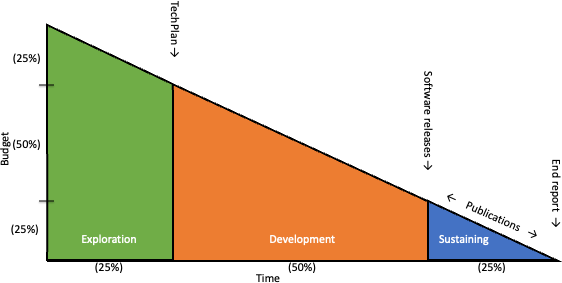
\includegraphics[scale=0.45]{img/budget-stages.png}
    %\caption{Project's budget breakdown}
    %\label{fig:project-budget}
\end{figure}

The eScience project team (including PM and RSEs) must submit their project hours in Exact by the end of each month. For
regular call projects, RSEs can write hours on awarded projects as soon as they are active in Exact, which in general
happens within a month of the project being granted. The PM writes management hours on the project budget.

Project hours are managed by different parties with different responsibilities:

\begin{table}[!h]
\begin{booktabs}{colspec={|>{\bfseries}m{0.2\textwidth}|m{0.8\textwidth}|},row{even}={nlesc-yellow}}
    \toprule
    Written by: &  Lead RSE, in collaboration with project team (including LA, TL), CMs, and others RSEs or colleagues (e.g. with relevant expertise on the subject), or relevant SIG. \\[1.5ex]
    Target audience: & Project team, TLs, PMs  \\[1.5ex]
    Schedule: &  %
    \begin{minipage}[t]{0.8\textwidth}
    \begin{itemize}\itemsep0em
        \item written at the start of the project work, before any software development starts,
        \item submitted to PM/TL by email before the deadline agreed during the project kick-off, 
        \item as a part of the project log (either full document in the log or a URL to it). 
    \end{itemize} 
      \end{minipage}
    \\[1.5ex]
    Approved by: & PM after due consultation of TL. \\[1.5ex]
    \bottomrule
\end{booktabs}
\end{table}

\bibliographystyle{abbrv}
\bibliography{references}

\end{document}
